\section{Methodik}

\subsection{Allgemeine Vorgehensweise}

\subsection{Extreme Gradient Boosting}

Extreme Gradient Boosting ist ein Verfahren aus dem Bereich des maschinellen Lernens, welches sich
in den letzten Jahren einer immer gr\"o{\ss}eren Beliebtheit erfreut hat~\cite{XGBoost}.
Die Grundlegende Funktionsweise dieses Verfahrens sei im Folgenden kurz beschrieben.

\subsubsection{Ausgangssituation}

Wir gehen davon aus, dass wir \"uber einen Trainingsdatensatz $\mathcal{D} = \{(\mathbf{x}_i, y_i)\}$
der Gr\"o{\ss}e $\left| \mathcal{D} \right| = n$ verf\"ugen, welcher aus den beobachteten Messungen $\mathbf{x}_i \in \mathbb{R}^m$
und der Zielgr\"o{\ss}e $y_i \in \mathbb{R}$ besteht, deren Wert wir vorhersagen wollen.

Das Ziel des Tree Boosting ist es, den Wert von $y_i$ durch ein Ensemble von Entscheidungsb\"aumen (CART)
vorherzusagen:
\begin{equation}
    \hat{y_i} = \phi(\mathbf{x}_i) =  \sum_{k=1}^K f_k(\mathbf{x}_i), \quad f_k \in \mathcal{F}
\end{equation}
Hierbei ist $\mathcal{F}$ die Klasse der besagten Entscheidungsb\"aume, welche in jedem ihrer $T$ Bl\"atter
einen konstanten Wert vorhersagen: $\mathcal{F} = \{f(\mathbf{x}) = w_{q(x)}\}$, wobei $q: \mathbb{R}^m \rightarrow T$
eine Funktion ist, die der Beobachtung $\mathbf{x}$ eines der $T$ Bl\"atter zuordnet und $w \in \mathbb{R}^T$ der Vektor
der Blattvorhersagen (Gewichte) des Baumes ist.

\subsubsection{Zielfunktion}

Die Zielfunktion, welche w\"ahrend des Trainings zur Anpassung des Modells minimiert wird, setzt sich wie folgt zusammen:
\begin{equation}
    \mathcal{L}(\phi) = \sum_{i=1}^n l(\hat{y}_i, y_i) + \sum_{k=1}^K \Omega(f_k)
\end{equation}
Hierbei ist $l$ eine differenzierbare und konvexe Verlustfunktion, welche Aufschluss \"uber die G\"ute der Vorhersage $\hat{y}_i$
liefert. Ein Beispiel ist der quadratische Fehler, welcher durch $l(\hat{y}_i, y_i) = (\hat{y}_i - y_i)^2$ gegeben ist.
Die Funktion $\Omega$ ist ein sogenannter Regularisierungs- oder Strafterm und ist wie folgt definiert:
\begin{equation}
    \Omega(f) = \gamma T + \frac{1}{2} \lambda \left \lVert w \right \rVert^2
\end{equation}
Das Ziel von $\Omega$ ist es, eine zu hohe Komplexit\"at der einzelnen Entscheidungsb\"aume in der Optimierung zu bestrafen und somit
w\"ahrend des Trainings simplere B\"aume zu bevorzugen. Dies geschieht mit dem Hintergedanken, eine \"Uberanpassung des Modells an
die Trainingsdaten verhindern zu wollen.
Der Parameter $\gamma$ bestraft hierbei die Anzahl der Bl\"atter $T$ eines Entscheidungsbaumes und der Parameter $\lambda$ bestraft
zu gro{\ss}e Gewichte in den einzelnen Bl\"attern.

\subsubsection{Training}

Das Grundprinzip des Boosting ist es, die Ensemble Modelle additiv nach dem Greedy-Prinzip zu trainieren.
Dies funktioniert hier so, dass die einzelnen Entscheidungsb\"aume nicht alle gleichzeitig angepasst werden, sondern
nach und nach zum Ensemble hinzugef\"ugt werden. Jeder Baum, welcher in einem Schritt hinzugef\"ugt wird, wird so trainiert,
dass er die Zielfunktion soweit wie m\"oglich minimiert.

Wenn im Optimierungsschritt $t$ also der Entscheidungsbaum $f_t$ zum Ensemble hinzugef\"ugt wird, ergibt sich die folgende
Verlustfunktion, welche durch $f_t$ minimiert werden soll:
\begin{equation}
    \mathcal{L}^{(t)} = \sum_{i=1}^n l(\hat{y}^{(t-1)}_i + f_t(\mathbf{x}_i), y_i) + \Omega(f_t)
\end{equation}
Die Regularisierungsterme $\sum_{k=1}^{t-1} \Omega(f_k)$ der bereits zum Ensemble hinzugef\"ugten B\"aume wurden hierbei weggelassen,
da sie im Zuge der Optimierung in Schritt $t$ nicht mehr ver\"andert werden k\"onnen.

\subsection{Regression mit ARMA-Fehlern}

\subsection{Validierung}

Die Aufgabe der Modellvalidierung ist es, Aussagen dar\"uber zu treffen, wie sich ein trainiertes Modell auf neuen und ungesehenen Daten
verhalten wird.
Ein bekanntes Verfahren zur Modellvalidierung ist die $k$-fache Kreuzvalidierung~\cite{elements}, welche auch in~\cite{IEEE} zum Einsatz
gekommen ist.
Hierbei wird der gesamte Datensatz zun\"achst zuf\"allig in $k$ gleich gro{\ss}e Partitionen unterteilt,
um im Anschluss das Modell jeweils auf $k-1$ Partitionen
zu trainieren und die \"ubrige Partition zum testen zu verwenden. Dies wird solange wiederholt, bis jede der
$k$ Partitionen genau einmal zum testen verwendet wurde.
Obwohl dieses Verfahren sehr weit verbreitet ist, gibt es in der vorliegenden Situation jedoch Anhaltspunkte daf\"ur,
dass sich die $k$-fache Kreuzvalidierung m\"oglicherweise als problematisch erweisen k\"onnte.

In Abbildung~\ref{fig:messfahrt-vodafone} ist eine der durchgef\"uhrten Messfahrten einmal beispielhaft zu sehen.
Man erkennt sofort, dass es sich bei den gemessenen Daten offenbar um eine Zeitreihe handelt.
W\"urde man in dieser Situation eine $k$-fache Kreuzvalidierung einsetzen, bei der die Daten zuf\"allig partitioniert werden,
so w\"urde der zeitliche Zusammenhang zwischen den Beobachtungen dadurch verloren gehen.
Es w\"are also fraglich, ob durch diese Art der Validierung verl\"assliche Aussagen \"uber das Modellverhalten auf zuk\"unftig
erhobenen Messdaten getroffen werden k\"onnen.
Aus diesem Grund wurde in diesem Projekt ein eigenes Validierungsverfahren eingesetzt, welches speziell auf die vorliegende Situation
zugeschnitten wurde.

\begin{figure}
    \centering
    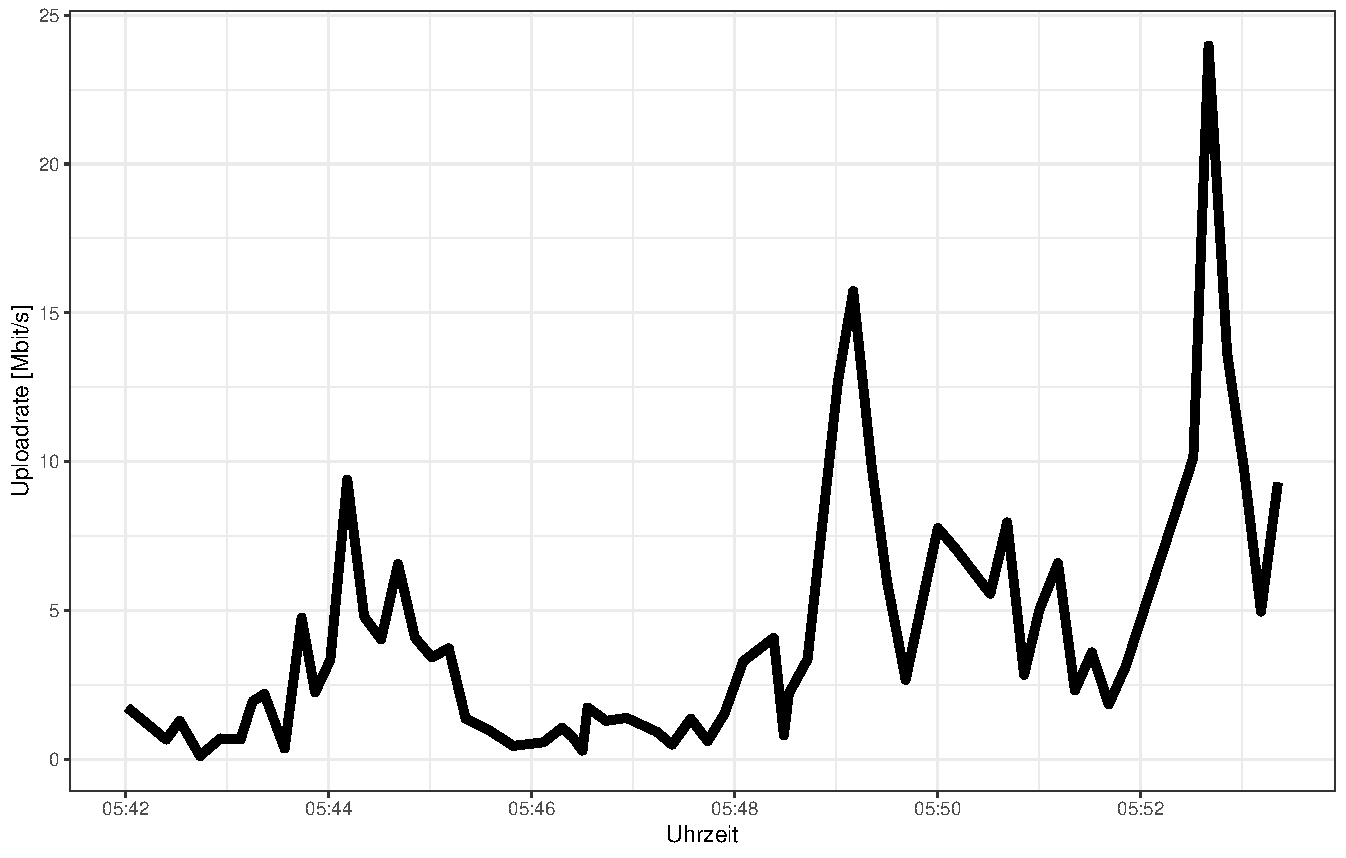
\includegraphics[width=0.8\textwidth]{abbildungen/highway_drive_vodafone}
    \caption{Die erste Messfahrt auf der Autobahn f\"ur den Netzbetreiber Vodafone am 12.12.2018.}
    \label{fig:messfahrt-vodafone}
\end{figure}

In Abbildung~\ref{fig:validierung} ist die in diesem Projekt eingesetzte Validierungsmethode einmal schematisch dargestellt.
Wie bereits beschrieben, besteht der gesamte Datensatz an Messungen f\"ur einen Netzbetreiber aus zehn einzelnen Messfahrten f\"ur
jedes der Szenarien \textit{campus}, \textit{highway}, \textit{suburban} und \textit{urban}.
Jeder dieser Fahrten kann also chronologisch eine Nummer von 1-10 zugewiesen werden, welche zusammen mit dem Szenario
eine Fahrt eindeutig identifiziert.
Im hier eingesetzten Validierungsverfahren wurde nun zun\"achst der gesamte Datensatz in zwei Teile aufgeteilt.
Der erste Teil besteht aus den Fahrten 1-7, der zweite Teil besteht aus den Fahrten 8-10.
In der Trainingsphase und beim Parametertuning kommt ausschlie{\ss}lich der erste Teil der Fahrten 1-7 zum Einsatz.
So wird sichergestellt, dass das Modell beim Training keine Informationen aus zuk\"unftigen Fahrten mit einbeziehen kann, wie
es beispielsweise bei der $k$-fachen Kreuzvalidierung der Fall w\"are. Fahrten 8-10 werden also ausschlie{\ss}lich zur Modellvalidierung
eingesetzt.

\begin{figure}
    \centering
    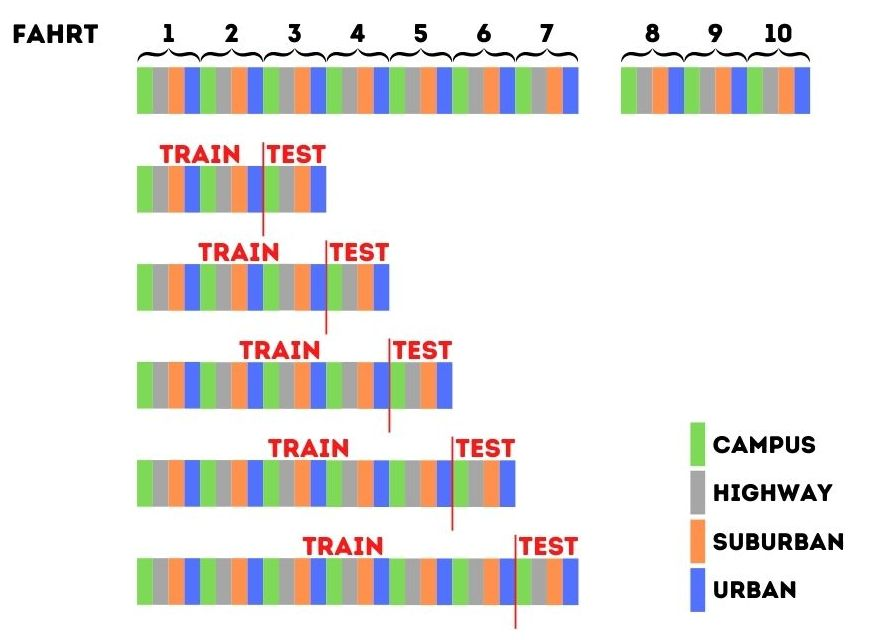
\includegraphics[width=0.8\textwidth]{abbildungen/validierung}
    \caption{Das eingesetzte Verfahren zur Modellvalidierung.}
    \label{fig:validierung}
\end{figure}

F\"ur eine geeignete Wahl der Hyperparameter werden auf dem Trainingsdatensatz, also Fahrten 1-7, verschiedene Parameterbelegungen
getestet und evaluiert. Zur Evaluation einer Parameterkombination kommt hierbei, wie sich in Abbildung~\ref{fig:validierung} ebenfalls
erkennen l\"asst, eine Art Kreuzvalidierung f\"ur Zeitreihen zum Einsatz. Hierbei wird der Trainingsdatensatz sukzessive um eine Fahrt
erweitert und immer auf der n\"achsten Fahrt getestet. Die ermittelten G\"utema{\ss}e werden dann im Anschluss \"uber die
Testdatens\"atze hinweg gemittelt.
